%!TEX root = ../Thesis.tex
\chapter{measureAbsorption}


\section{Studies to test peptide absorption}
The overall goal for an oral formulation is to achieve a high bio-availability with low a variance. That is to maximize the percentage of dose absorbed, and to minimize the day-to-day variance. However in order to learn how a formulation attempt may be failing, it is needed to break down the process into individual steps. The typical three steps to consider are dissolution of the tablet, enzymatic stability and permeation enhancement. The article first article, \textit{"The role of citric acid in oral peptide and protein formulations: Relationship between calcium and proteolysis inhibition."} \cite{welling2014citric}, included in this thesis is good example of the \textit{in vitro} methods used to evaluate permeation enhancement and enzymatic stability. First the three steps can be understood as a link. If one is failing the overall result will be poor.

Studies to test permeation enhancement ranging from early proof-of-concept development to clinical trials late every are listed in Figure \ref{typeOfExperiment}. Beyond this list focusing on peptide permeation studies, also dedicated studies of \textit{in vitro} dissolution, peptide stability and toxicology would e.g. be required.

((membrane transport/electrical resistance image?))

In preclinical development, studies are formally segregated in two categories the \textit{ex vivo} outside the living and the \textit{in vivo} inside the living organism. Often \textit{in vivo} refer to animal studies, not human. The term \textit{in vitro}, in reagent glass, is used instead of \textit{ex vivo}. Speaking of \textit{in silico}, in silicium, is used for computer models. One may feel the latin buzzword terminology has been overly used to a point no longer being \textit{in}. Further there are clinical trials in human. It is obviously sensible to test many new insulin analogues and formulations in fairly inexpensive and fast studies. The three main properties of oral formulations to optimize are named  solubility, enzymatic stability and epithelial permeability. Most medical research observe and propose general causal mechanisms. Where clinical trials can be very representative for the intended population of patients, it is difficult to learn exactly why a therapy elicited no positive result. The multiple potential steps of failure cannot be observed. Moreover, negative confirmation is important to narrow in what part of a therapy is essential for a positive outcome. Ethical considerations limit clinical trials to prescribe therapies to patients in conflict with their best self interest. With \textit{in vivo} studies it is possible to test treatments as long as the animal suffering is kept minimal. Still the gastro-intestinal tract is a complicated machinery and it is not possible to control or measure every aspect the peptide absorption process. Moreover other sources of variance such as the individual variance in animal physiology may introduce noise into measurements. The animal variance makes a step-wise incremental optimization of formulation challenging, as it becomes hard to evaluate what works, due to no significant change of bioavailability. The lab bench \textit{in vitro} experiments offers close to full control of the experiment conditions. These experiments are often fast and or of low cost, while the reproducibility and statistical power are high. From a modeling perspective a larger set observations number is needed, especially for non-linear machine learning, see \ref{some section}. Therefore to get hands on a large set of \textit{in vitro} data is more easy. The \textit{in vitro} experiments can often be crude and it is accepted as a necessary evil, that the conditions do not exactly represent completely a clinical situation. Figure \ref{typeOfExperiment} listing the range of permeation experiments, is intended reflect this conflict between representative studies and elucidating studies.
When training machine learning models on data from \textit{in vitro} experiments, we only expect the model to reflect the experiment. With a hopefully sufficient theoretical understanding of the overall peptide absorption and the various biases of the \textit{in vitro} experiments, we can hopefully place the model in a context to obtain useful predictions and identify potential causal relationships between formulation and outcome.

\subsection{Caco-2 monolayers}
Caco-2 monolayers have been a standard screening method for intestinal drug permeability. The Caco-2 permeation model, as other permeation models, consist of a donor chamber, an epithelial barrier and a reciever chamber. Caco-2 monolayers are colonic human cancer cells, which a much more prolific and easy to handle, than primary epithelial cells. When seeded on a 2 cm in diameter micro porous filter on a 12-well plate, the Caco-2 cell line will grow and form a epithelial monolayer in two weeks. A typical test will use 4 monolayers per tested treatment and the study is to be repeated on a different day. During the test, the nutrient reach growth media is replaced with a minimal buffer solution. The buffer solution only contain a physiological level of electrolytes such as calicium, potassium, sodium, chloride and phosphate plus an acid/base buffer. These ions maintain isotonicity and a normal electrical membrane potential. Active membrane transporter receptors in the epithelial membrane rely on a given correct membrane potential. Within standard drug development of small molecules, a low permeability result would likely lead discarding the given analogue, as it easier to find a new analogue with a favorable permeability. In insulin therapy, there are few alternatives to insulin-like analogues and therefore the low permeability must alleviated by formulation. To use Caco-2 monolayers to test absorption enhancers for oral peptide delivery make up, just a small part of the use of Caco-2 monolayers. Here the permeability of insulin is already low, and may be increased by a given absorption enhancer. For surfactant enhancers at high concentration, the monolayer can become completely disrupted, while at low concentration no useful effect is observed.

\subsection{Measuring permeability}
To estimate how potent an permeation enhancer is, permeation markers have been used. An obvious marker is human insulin itself, but insulin is difficult to handle and quantification by immuno-assay can be expensive. A number of of alternative permeation markers are typically used to substitute or compliment insulin. One of these are $^{14}$C or $^3$H isotope labeled mannitol. Mannitol, approximately as hydrophilic as glucose, is thought to only diffuse passively via the paracellular pathway through the tight-junctions \cite{anderberg1992epithelial,artursson1994effect}. Unlike glucose, mannitol is not taken up by active transport, and is therefore suitable passive transport marker. As Mannitol is hydrophillic it cannot permeate the lipophilic plasma membrane and can only diffuse between the cells by the tight junctins. Therefore is mannitol a para-celullular passive permeation marker. Besides permeation of mannitol through the tight junctions, also permeation of electrolytes can be used as a marker of how open the junctions currently are. Trans epithelial electrical resistance (TEER) can measure how open the paracellular tight junctions are, as the junction cross sectional area is proportional to the conductivity, and conductivity is inverse resistance. TEER is the easiest non-invasive measurement to apply. Lowering the epithelial resistance e.g. 50\% with an absorption enhancer will likely translate to a (?-fold increase) of permeability of both mannitol and insulin. FITC-dextran 4000 dalton (FD4) is a florescent labeled sugar polymer of similar hydrophilicity and size as insulin. FD4 can mimic insulin as transport marker as it has the molecular weight and hydropphlicity (citation). FD4 on the other hand has no enzymatic instability (does it not?) and can be used to estimate what would have been the permeation of unchanged insulin, if the has been no enzymatic cleavage in the luminal space. FD4 can be specifically and accurately quantified, as it is a fluorophore.

\begin{figure}[ht]
\label{devel_typeOf}
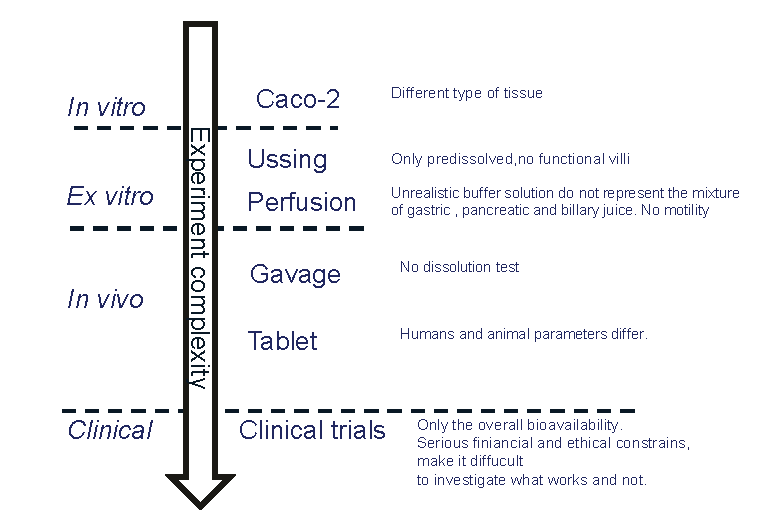
\includegraphics{graphics/typeOfExperiments.pdf}
\caption{Schematic overview of types of experiments ranging from Caco-2 to clinical. Simple experiments to not accurately simulate the actual process, and there will be a number of biases which must not be over interpreted.}
\end{figure}


\subsection{Calculating permeability}
Gradient driven diffusion of mannitol, FD-4 and insulin across the epithelial barrier is a first order process where the transport per time is proportional to the concentration gradient $C_i$ ($mol/L$). Only a few percent of the total amount of transport marker will permeate the barrier and therefore will $C_i$ be approximately unchanged throughout the experiment. Hereby becomes the apparent permeability $P_{app}$ proportional to the transport rate or flux $J$ ($mol/s$) which is usually estimated by sampling the reciever basolateral side 4 to 6 times. When plotting reciever concentration versus time, a fitted ordinary least squares slope is used as the overall transport rate through out the experiment. Permeability is corrected for the cross sectional area of the chamber. The permeant flux $J$ is expected to be proportional to the cross sectional area of the chamber $A$ (cm$^2$). Therefore the apparent permeability is  calculated as

$P_\{app\} = J/A/C_i = \frac{dC_r}{dt}/A/C_i \quad ,$

where $\frac{dC_r}{dt}$ is the slope of ordinary least squares regression of receiver chamber concentration versus time. The intercept with x-axis (time) is interpreted as the lag time, the time it takes saturate the mucus layer, the thin unstirred water layer and the epithelial junctions. The lag time is typically a couple of minutes depending weather using Caco-2 or Ussing chamber. To observe a apparent constant flux e.g. throughout a one hour experiment is normal. The small decrease in concentration gradient of some few percent throughout the study, may theoretically have caused deceleration of the flux. However, it is possible that the actual permeability of the epithelial barrier is increasing through the one hour flux study due to slow deterioration by the absorption enhancer, and therefore a constant flux is observed. In control epithelial barriers without absorption enhancer treatment, the barrier integrity is not expected to decline, but at the same time the flux is very low, so the concentration gradient do not change.

\begin{figure}[ht]
\label{meassure_TEERPapp}
\includegraphics[width=\textwidth,height=\textheight,keepaspectratio]{graphics/sketch_measuring_permeability.png}
\caption{Illustration of how \textit{(a)} P$_{app}$ and \textit{(a)}  TEER is calculated.}
\end{figure}


The tight junctions are in ideally water filled channels with a given specific conductance of the solute. When tight junction are widened, the cross-sectional area of tight-junction per area tissue is changed. Similarly as marker transport is driven by a concentration difference, the electrical current $A_{e}$ (Ampere $A_c$) is driven by an electrical potential difference $U$ (Voltage V). The tissue conductivity $S$ corrected for area tissue $S_A = S/A$, is the equivalent to $P_{app}$. The inverse electrical ion permeability is described in TEER (trans epithelial electrical resistance). TEER (Ohm cm$^2$) is the inverse $S_A$.

$\frac{1}{RA} = S_A = A_e/A / U \quad.$

To summarize both $P_{app}$ and inverse TEER both describe how readily a flux of either molecules or ions are driven through the epithelial barrier by respectively a concentration gradient or a electrical potential gradient. $P_{app}$ is measured by maintaining a constant concentration gradient determining the molecular flux. TEER is either measured with voltage or current clamping. To measure TEER with voltage clamping is to control the electrical gradient (potential difference) with electrodes and measure the actual current. Current clamping is oppositely to drive a specified flux of ions (current) through the epithelial barrier and record the electrical gradient. TEER reflects the inverse para-cellular permeability of the epithelial barrer. For direct measurement of permeability of a given drug molecule, TEER is mainly used to check barrier integrity. For measuring the potency of permeation enhancers to increase permeability, TEER can be used as indicator hereof. To directly measure the permeation of insulin would be preferable, but this is more slow, expensive and unlikely to find in already published results. As the current and potential difference can be manipulated with electrodes, the time resolution for TEER measurements are in seconds. The time resolution for permeation markers is limited by the sampling rate and accuracy of the concentration determination. The sampling rate of Caco-2 studies are typically once per 15 minutes.

\begin{figure}[ht]
\label{devel_fassif}
\includegraphics[width=\textwidth,height=\textheight,keepaspectratio]{graphics/devel_Fasssif_PCC2.png}
\caption{Single figures copied from \cite{tippin2008biorelevant,nawroth2011liposome} to illustrate why the potency of lipophilic permeation enhancers are likely overestimated in in-vitro studies using surfactant free buffers. Palmitoyl carnitine was found by Tippin \textit{et al} to be 12 times less potent in a Fassif buffer with Taurocholate and lechitine an EC$_{50}$}
\end{figure}

\section{Mechanisms of absorption enhancement in oral formulations}

The formulation part of oral peptide therapy is mainly to ferry the highest possible total and relatively amounts of insulin unchanged through the upper gastro-intestinal tract. The two major barriers are enzymatic degradation and poor epithelial permeability. Other barriers are the mucus and thin unstirred water layer on top of the epithelia. These barriers are not regarded as prominently rate limiting bottle necks and are not given as much attention.(cite)

\subsection{Preventing and measuring enzymatic degradation}
Enzymatic stability of peptides/proteins very greatly in the intestinal tact. From dissolution in the small intestinal lumen the window is concidered to be from a single minute upto 15 minutes(citation somastatin). Enzymatic degradation rate ($V_i$) is assumed to follow Michalis-Menten kinetics. Describing the degradation rate per enzyme as a function of substrate/peptide concentration $[S]$, enzyme-substrate binding constant ($K_m$), and max enzyme degradation speed $V_max$.

$V_i = \frac{V_{max} [S]}{K_{M}+[S]}$

The MM kinetics describe that at very low concentrations of substrate the degradation rate will be proportional to the concentration of insulin in the luminal space, thus a first order decay process. 
The Michaelis-Menten kinetics opens for three ways to limit relative peptide degradation. First the apparent $K_m$ binding constant can be increased by adding a competitive substrate. The enzyme will then bind to another substrate such as soy bean peptides or Bowman-Birk compounds. A very potent non competitive inhibitor would bind strongly to the enzyme, such that only a small amount of inhibitor would be needed. Such non-peptide inhibitors are in practice toxic and not suited for chronic treatment \cite{bernkop1998use} \cite{murthy1980effect}. 

The second option which is used in the first article \cite{welling2014citric} of this thesis is to lower the apparent $V_max$ the intrinsic fastest rate of enzyme conversion. Citric acid itself is not a substate of the trypsin and chymotrypsin. As citric acid is dissolved, it will partly release protons into the luminal space and thereby lower pH. The enzymes trypsin and chymotrypsin has an 10-fold lower $V_max$ at pH=4. At pH 3 trypsin denatures 95\% over 30 minutes.
The last why to inhibit the relative degradation is to release as much substrate as fast possible into the luminal space. As the substrate concentration increase $[S] >> K_m$ and $V_i \approx V_{max}$ there will be a theoretical upper limit for how much insulin can be degraded per time. Driving up the concentration of insulin, well surpassing the linear range of degradation and approach the $V_max$. This appraoch could fairly be called hit and run, that so much insulin is realsed in such a short concentration in time and location, that the enzyme can't degrade all at once. The ladder approach is highly connected to the dissolution of the tablet. If the tablet disolves over an hour. The insulin would be released very slowly in small concentrations, and the enzymes will have plenty of opportunity to degrade all insulin. To simply only drive up the amount of insulin included in a tablet is not likely to be the solution alone, as the insulin is very costly to produce. Also, due to drug safety, there can be a upper boundary of how much insulin can be included in one tablet, as it may lead to an overdose and acute hypoglychemia if suddenly a large fraction insulin was absorbed in patient.

Citric acid is one approach to lower the 
Substrate inhibition with so


\subsection{}

\section{Article: The role of citric acid in oral peptide and protein formulations:
Relationship between calcium chelation and proteolysis inhibition}

\newpage

\includepdf[pages={1-},scale=0.90,pagecommand={\pagestyle{myruled}}]{chapters/citricAcid.pdf}


Discuss fast and slow release of tablet in respect to degradation constants. Solubility

Discuss 